%%
%% using aastex version 6.3
%% Setup

\documentclass[linenumbers]{aastex631}

\newcommand{\vdag}{(v)^\dagger}
\newcommand\aastex{AAS\TeX}
\newcommand\latex{La\TeX}


\begin{document}

\title{The Morphology of the Stellar Remnant of the Milky Way + M31 Major Merger}

%% Author

\author{Hanga Andras-Letanovszky}
\affiliation{Department of Astronomy, University of Arizona,  933 N Cherry Ave, Tucson, AZ}

%% Introduction

\section{Introduction}

% Define your proposed topic and how it relates to galaxy evolution
The topic I will be investigating in this project is the morphology of a galaxy merger remnant, specifically one formed in a "dry" major merger between two gas-poor spiral galaxies of roughly equal masses. 
The remnant is the stars and gas from both galaxies that remained gravitationally bound post-merger, and its properties are heavily influenced by the properties of the parent galaxies as well as how the collision occurred \citep{Barnes+1992}. 
An example of a (simulated) merger event can be seen in Fig. \ref{fig:merger}, with the remnant shown at t=2.66 Gyr.
In particular, the morphology, or shape, of the galaxy is determined by the aforementioned factors.
This shape is broadly described in terms of whether it is more disk-like or elliptical; in the former case, whether spiral arms are present is important, and in the latter, whether it is more spheroidal or elongated.
Inherently collisional structures such as tidal arms and bridges are also often observed, and these in particular frequently help identify galaxies formed in mergers \citep{Duc2013}.
\begin{figure}[h!]
    \centering
    \centering
    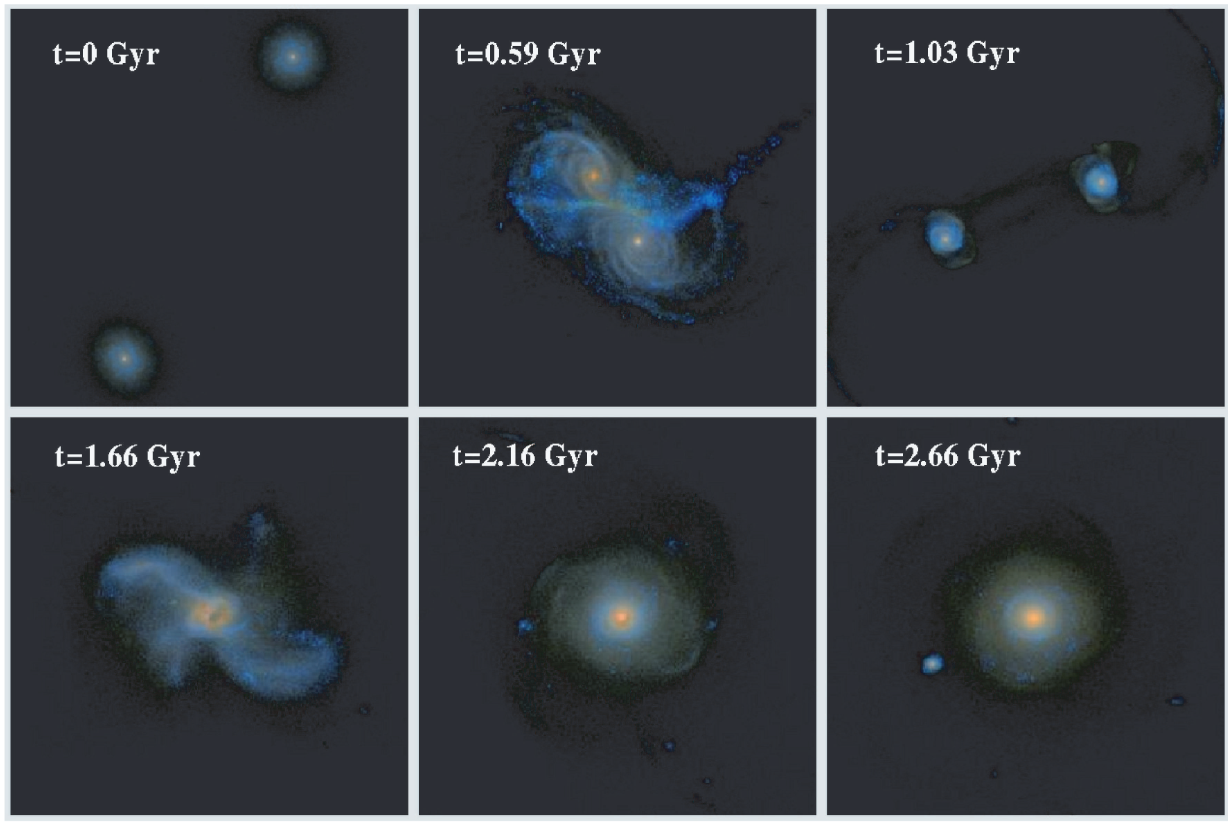
\includegraphics[width=0.5\linewidth]{merger.png}
    \caption{
        A simulated merger of two Sbc galaxies from \cite{Lotz+2008}.
        From right to left, the top row shows the two undisturbed pre-merger progenitors, the first pass, and the maximal separation after the first pass.
        The bottom row shows the merger of the nuclei of the galaxies, the remnant 0.5 Gyr post-merger, and the remnant 1.0 Gyr post-merger.
        }
    \label{fig:merger}
\end{figure}

% State why this topic matters to our understanding of galaxy evolution
Studying the morphology of galaxy merger remnants is incredibly important for understanding galaxy evolution because most galaxies are affected by mergers and interactions \citep{Barnes+1992}.
For one, knowing how merger remnants look will aid us in identifying past merger events both nearby and at higher redshifts, helping us constrain merger rates and timescales throughout the history of the universe \citep{Lotz+2008}. 
This will help us understand both the percentage of galaxies that undergo merger events and how many events they undergo.
Collisional debris, such as tidal tails, even have potential as a method of dating mergers \cite{Duc2013}.
Additionally, as stated before, the morphology of the remnant is heavily influenced by the properties of the parent galaxies and the collision itself, so knowing precisely how the morphology changes with these factors can allow us to glean information about the progenitors of a remnant, further elucidating the galactic evolution process \citep{Barnes+1992}.
In particular, we care about major merger events between spirals because they are thought to be a significant formation route for elliptical and spheroidal galaxies \citep{Barnes+1992}, as they're very commonly found in dense clusters. 
As such, these galaxies are often used to trace past merger events; however, there are other potential formation pathways for ellipticals and spheroids, such as "inside-out growth" consisting of more minor mergers that must be accounted for \citep{Lotz+2008}.
Thus, studying the morphology of major merger remnants will help us to better distinguish between ellipticals and spheroids formed via major mergers from those formed in other ways, allowing us to see the true prevalence of major mergers in elliptical galaxy formation and better understand the link between spirals and ellipticals.

% Overview of our current understanding of the topic in galaxy evolution
As it stands, we know a fair amount about how the properties of the progenitor spirals affect the morphology of the remnant.
The kinematics of the merger are one important factor; a merger of two galaxies with high orbital angular momentum tends to produce oblate, rapidly rotating spheroids --- this is true in general in any case where the parent galaxies merge in a way that leaves the remnant with a high angular momentum --- whereas head-on collisions usually create prolate spheroids \citep{Barnes+1992}. 
Similarly, prograde orbits pre-merger usually leave remnants with long, narrow tidal tails, as opposed to the shorter, more diffuse plumes associated with retrograde orbits \citep{Duc2013}. 
The dark matter halos of the merging galaxies also play a vital role in the merger, as their interactions with each other actually cause the most angular momentum loss. 
Generally, the progenitors' disks and bulges will also lose most of the their angular momentum to interacting with their own disturbed halos, only really interacting with the disk and bulge when they collide and merge; this is why remnants tend to still have dense, luminous central bulges \citep{Barnes+1992}.
The gas content of the parent galaxies is another crucial determinant of the remnant morphology.
In particular, gas-poor, or "dry," galaxy major mergers tend to produce rounder, more elliptical remnants, whereas gas-rich ("wet") major mergers tend to produce more oblate, disk-like galaxies.
This occurs due to the the fact that as the gas acquires angular momentum during the merger, it tends to flatten out into a rotating disk at the center \citep{Eliche-Moral+2018}.
On the other hand, large bulges tend to be more conducive to forming massive ellipticals \citep{Barnes+1992}.
Generally, it's thought that the vast majority of major mergers between spirals create ellipticals; however, simulations such as those by \cite{Eliche-Moral+2018} have shown that these mergers can create significant amounts of very oblate, disk-like remnants, even as far as S0 galaxies on the borderline between ellipticals and spirals, despite concerns that major mergers were too "catastrophic" to allow for an ordered disk to form, as shown in Fig. \ref{fig:morphs}.
\begin{figure}
    \centering
    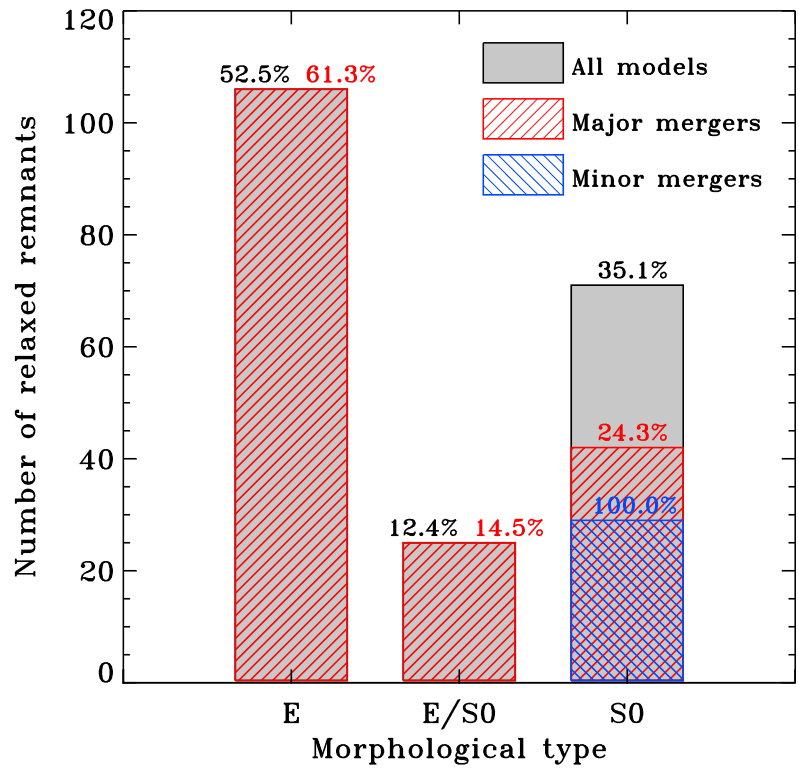
\includegraphics[width=0.5\linewidth]{morphs.png}
    \caption{
        Distribution of remnant morphological types across a sample of 202 merger simulations from \cite{Eliche-Moral+2018}.
        Percentages shown are calculated with respect to the total sample, as well as the samples of major mergers and minor mergers separately.
        Ellipticals dominate, but S0 types are more prevalent than expected.
        }
    \label{fig:morphs}
\end{figure}
    
% What are the open questions related to this topic?
There are still many questions left unanswered relating to major mergers and remnant morphology, though. 
For example, what is the precise relationship between bulges and ellipticals? 
What is the complete range of remnant dynamics and orbital structures that can be produced by a merger?
What are the exact roles played by mergers and and other evolutionary mechanisms in transforming spirals into elliptical, spheroidal and S0 galaxies?
Is more discrete formation through mergers preferred, or more continuous methods like cold gas accretion?
How does this change with redshift?
Questions like these are the ones that full simulations of mergers and careful analysis of the morphology of the remnant will be able to answer, especially in the era of abundant JWST data of high redshift galaxies.


\section{Proposal}

\subsection{This Proposal}

I will investigate two related questions using the simulation in \cite{van_der_Marel-2012}:

1. Is the 3D structure of the remnant a spheroidor does it have some elongation or triaxiality?

2. How does the shape of the remnant vary as a function of radius?

\subsection{Methods}

I will perform the following analysis for 2 different snapshots of both M31 and the Milky Way (MW). 
The first will be 2 Gyr after the merger occurs (Snap Number 595), so I can compare the result with the prediction that relaxed S0 remnants can form roughly 1 -- 2 Gyr after the merger occurs.
I will also look at the very last available snapshot (Snap Number 801) to see how or if the remnant relaxed significantly in the intervening time.
In both cases, I will use high-resolution snapshot files so that I can get as accurate a picture of the structure of the remnant as possible.

The first step will be to find the center of mas (CoM) of the remnant. 
To do so, I will first define the CoMs of M31 and MW separately using the \texttt{CenterOfMass} class from Homework 4. 
For simplicity, I will assume the disk particles accurately trace the CoM of the bulge particles as well, and thus only use disk particles in the CoM calculation. 
(It's important to note, however, that the disk and bulge could in theory have different CoMs).
To get the CoM of the remnant ($R_r$), then, I will calculate the center of mass of the M31 and MW CoMs ($R_{M31}$ and $R_{MW}$ respectively):

\begin{equation}\label{eq:CoM}
    R_r = \frac{M_{MW}R_{MW} + M_{M31}R_{M31}}{M_{MW}+M_{M31}}
\end{equation}

My next step will be to make the actual remnant object that I will analyze. 
To do so, I will read in the positions and velocities of the disk and bulge particles of both M31 and MW, and then concatenate them into one position and one velocity array, each containing the disk and bulge particles of both galaxies.
Subtracting the remnant CoM position and velocity from the relevant arrays will then yield the needed CoM-relative positions and velocities. 
Finally, I will use these positions and velocities with \texttt{RotateFrame()} from Lab7 to rotate the remnant such that its angular momentum is aligned with the z-axis.
This will allow me to observe the remnant "edge-on" and "face-on."
\begin{figure}[h!]
    \centering
    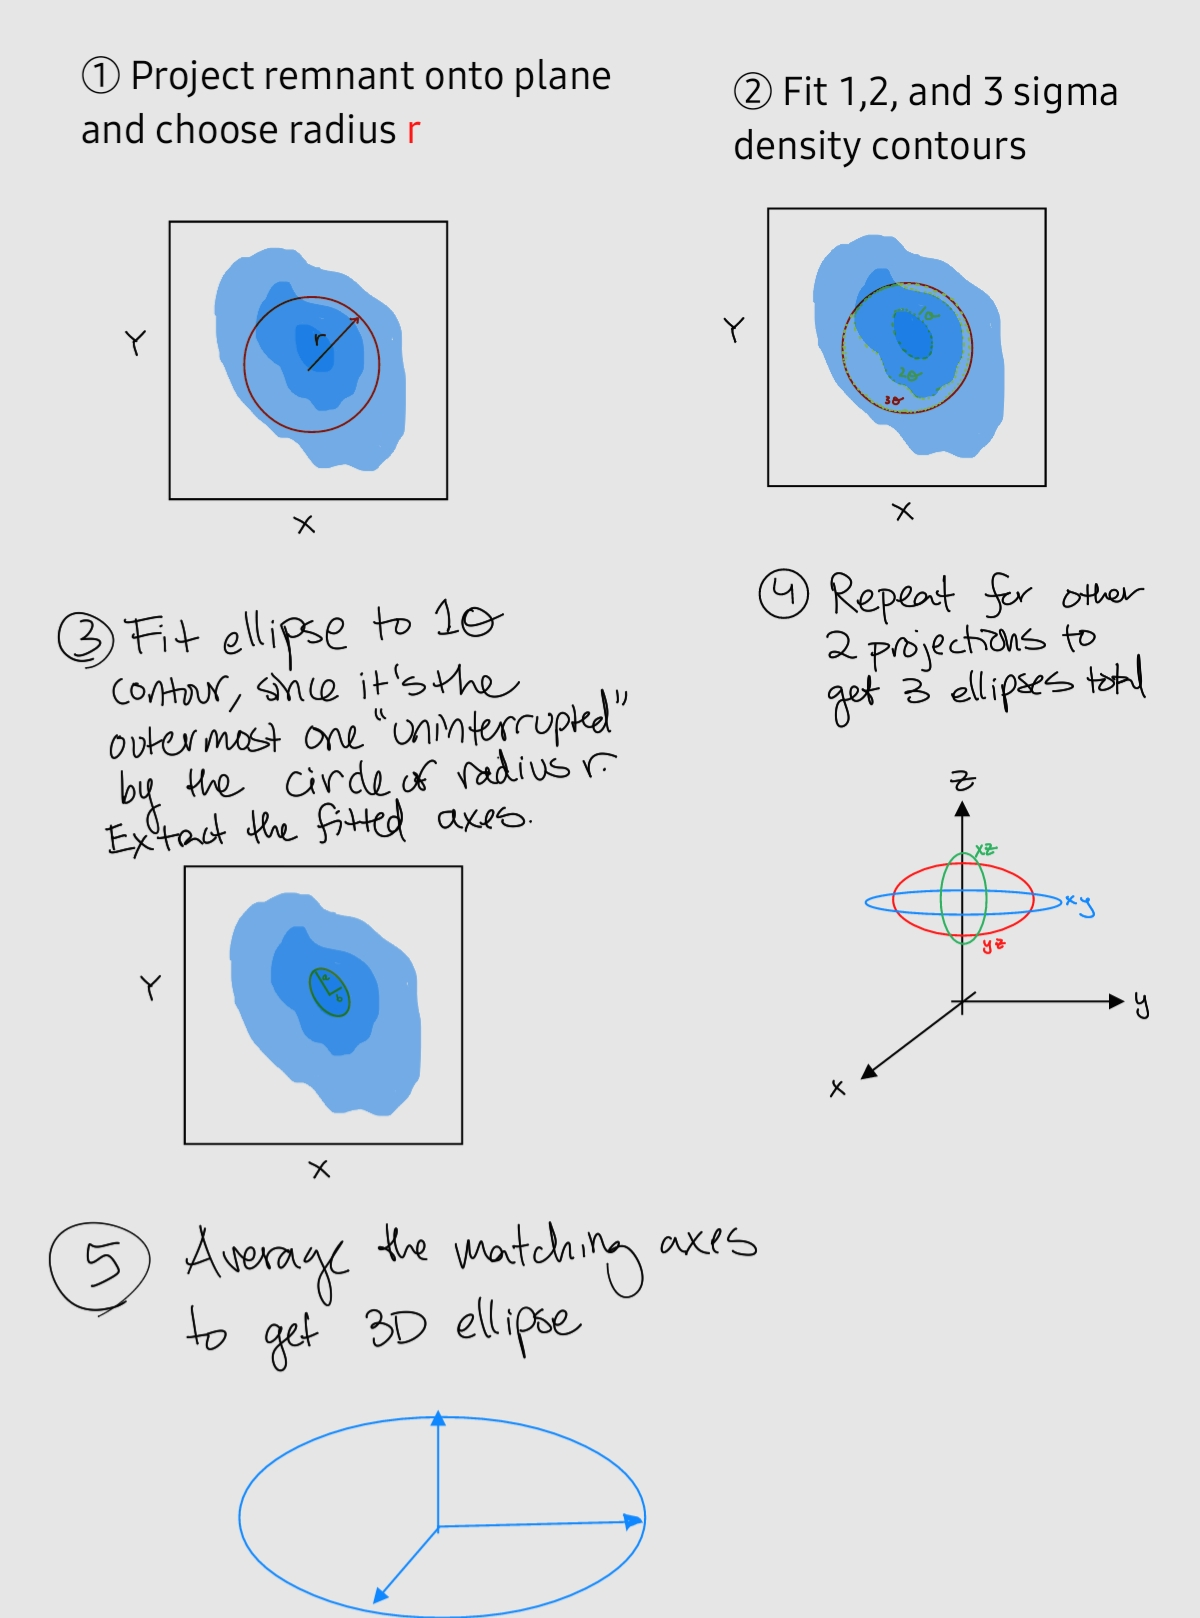
\includegraphics[width=0.5\linewidth]{Methods.jpg}
    \caption{
        A visualization of the process of finding the 3D structure of the remnant within some radius $r$.
    }
    \label{fig:methods}
\end{figure}

The following steps, which are pictured in Fig. \ref{fig:methods}, I will repeat for the projection of the remnant onto the xy, yz, and xz plane to get a full picture of the 3D structure of the remnant.
First I will choose some radius $r$ within which to analyze the shape of the galaxy. 
I will first select only particles that fall within that radius $r$. 
Using \texttt{density\_coutour()} from Lab 7, I will then fit 1$\sigma$, 2$\sigma$, and 3$\sigma$ contours to these particles to show the particle density structure.
I will then choose the contour that traces the outermost "shape" of this part of the galaxy, i.e. the outermost contour that traces a distinct shape and doesn't just trace the circle described by $r$. 
From there, I will fit an ellipse of the form 
\begin{equation}
    \frac{(x\text{cos}\theta + y\text{sin}\theta)^2}{a^2} + \frac{(x\text{sin}\theta + y\text{cos}\theta)^2}{b^2} = 1
\end{equation}
where $a$ is the semimajor axis, $b$ is the semiminor axis, and $\theta$ is the tilt of the ellipse, to the particles nearest to the chosen contour using least-squares fitting.
By calculating $a$ and $b$ for all three projections, I will be able to average the projected axes to approximate the three axes of the ellipsoid shape of the galaxy within that radius, $A$, $B$, and $C$, which satisfy

\begin{equation}
    \frac{z^2}{A^2} + \frac{y^2}{B^2} + \frac{x^2}{C^2} = 1 .
\end{equation}
Then, finally, I will be able to classify the shape of the ellipsoid as \textit{spheroid} ($A \approx B \approx C$), \textit{oblate} ($A \approx C > B$), \textit{prolate} ($B > C \approx A$), or \textit{triaxial}, where the axes are all different lengths. 
I will repeat this process for a range of radii, starting from a little above where the bulge seems to end to a little past the furthest remnant particle.

\subsection{Hypothesis}

My hypothesis is that the remnant will be spheroidal, or maybe slightly oblate, but certainly not as oblate or disk-like as an S0 galaxy. 
M31 and the Milky Way are both rather gas-poor galaxies residing in the "Green Valley," so I do not expect them to have enough gas to allow the disk to reform post-merger, even in the much later of the two snapshots.


%% Bibliography!

\bibliography{biblio}{}
\bibliographystyle{aasjournal}


\end{document}

